\documentclass{article}
\usepackage[a4paper, total={6.5in, 9in}]{geometry}
\usepackage[brazil,portuges]{babel}
\usepackage[utf8]{inputenc}
\usepackage[T1]{fontenc}
\usepackage{lmodern}
\usepackage{amsmath}
\usepackage{indentfirst}
\usepackage{titlesec}
\usepackage{todonotes}
\usepackage{enumitem}
\usepackage{tikz}
\usepackage{amsmath}
\usepackage{amsfonts}
\usepackage{amssymb}
\usepackage{gensymb}
\usepackage{array}
\usepackage{amsmath}
\usepackage{indentfirst}
\usepackage{titlesec}
\usepackage{todonotes}
\usepackage{enumitem}
\usepackage{tikz}
\usepackage{array}
\usepackage{subcaption}
\usepackage{listings}% http://ctan.org/pkg/listings
\lstset{
	basicstyle=\ttfamily,
	mathescape
}

\title{CG - Lista de Exercícios 2}
\author{André L. Mendes Fakhoury}
\date{2021}

\begin{document}

\maketitle

Nascimento: Dia $D = 17$, Mês $M = 4$

\section{As matrizes Model, View e Projection utilizam transformações geométricas 3D para compor as coordenadas de mundo, visão e clip. Esse processo também é chamado de pipeline do Viewing 3D. Escreva, com suas palavras, a função de cada etapa do pipeline.}

Originalmente, os objetos estão em seu espaço original, denominado espaço local (por exemplo, podemos fixar a localização de cada objeto para ficar centrado na origem). Então é aplicada a matriz Model, para realizar as transformações (escala, translação, rotação, ...) para o denominado espaço Mundo. A partir disso, é aplicada a matriz View para delimitar o que o observador enxerga da cena, e depois disso é aplicada a matriz Projection, para dar as noções de projeção. Como utiliza-se as coordenadas homogêneas, a posição final de cada vértice dos objetos é descrita como:
$$P' = \text{Projection} \cdot \text{View} \cdot \text{Model} \cdot P$$

\begin{figure}[h!]
	\centering
	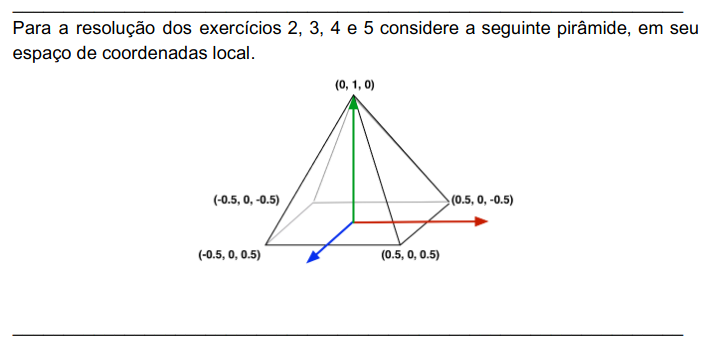
\includegraphics[scale=0.6]{img/piramide.png}
\end{figure}

\section{Apresente a matriz Model para transladar a pirâmide '-M' no eixo z, ou seja, para posicionar a pirâmide mais ao “fundo” no espaço de mundo. Apresente as coordenadas da pirâmide no espaço de mundo.}

A matriz translação é a seguinte:

$$M =
\begin{pmatrix}
1 & 0 & 0 & t_x\\
0 & 1 & 0 & t_y\\
0 & 0 & 1 & t_z\\
0 & 0 & 0 & 1
\end{pmatrix}$$

Como iremos transladar apenas $-4$ no eixo-z, temos:

$$M =
\begin{pmatrix}
1 & 0 & 0 & 0\\
0 & 1 & 0 & 0\\
0 & 0 & 1 & -4\\
0 & 0 & 0 & 1
\end{pmatrix}$$

Aplicando em cada vértice da imagem:

$$V_1' = \begin{pmatrix}
	1 & 0 & 0 & 0\\
	0 & 1 & 0 & 0\\
	0 & 0 & 1 & -4\\
	0 & 0 & 0 & 1
\end{pmatrix} \cdot \begin{pmatrix}
0\\
1\\
0\\
1
\end{pmatrix} = \begin{pmatrix}
0\\
1\\
-4\\
1
\end{pmatrix}$$

$$V_2' = \begin{pmatrix}
1 & 0 & 0 & 0\\
0 & 1 & 0 & 0\\
0 & 0 & 1 & -4\\
0 & 0 & 0 & 1
\end{pmatrix} \cdot \begin{pmatrix}
0.5\\
0\\
-0.5\\
1
\end{pmatrix} = \begin{pmatrix}
0.5\\
0\\
-4.5\\
1
\end{pmatrix}$$

$$V_3' = \begin{pmatrix}
1 & 0 & 0 & 0\\
0 & 1 & 0 & 0\\
0 & 0 & 1 & -4\\
0 & 0 & 0 & 1
\end{pmatrix} \cdot \begin{pmatrix}
0.5\\
0\\
0.5\\
1
\end{pmatrix} = \begin{pmatrix}
0.5\\
0\\
-4.5\\
1
\end{pmatrix}$$

$$V_4' = \begin{pmatrix}
1 & 0 & 0 & 0\\
0 & 1 & 0 & 0\\
0 & 0 & 1 & -4\\
0 & 0 & 0 & 1
\end{pmatrix} \cdot \begin{pmatrix}
-0.5\\
0\\
0.5\\
1
\end{pmatrix} = \begin{pmatrix}
-0.5\\
0\\
-4.5\\
1
\end{pmatrix}$$

$$V_5' = \begin{pmatrix}
1 & 0 & 0 & 0\\
0 & 1 & 0 & 0\\
0 & 0 & 1 & -4\\
0 & 0 & 0 & 1
\end{pmatrix} \cdot \begin{pmatrix}
-0.5\\
0\\
-0.5\\
1
\end{pmatrix} = \begin{pmatrix}
-0.5\\
0\\
-4.5\\
1
\end{pmatrix}$$

E estes $V_i', i \in \{1, 2, 3, 4, 5\}$, são as coordenadas no espaço mundo.


\section{Apresente uma matriz View, com parâmetros definidos por você, e as coordenadas da pirâmide no espaço de Visão.}

Uma possível matriz View pode ser definida com os seguintes parâmetros:

\begin{lstlisting}
camera_pos = $P_0$ = $(x_0, y_0, z_0)$ = (0, 0, 5)
camera_target = $\vec T$ = (0, 0, 0)
camera_up = $\vec V$ = (0, 1, 0)
\end{lstlisting}

Com estes parâmetros, temos os vetores $u, v$ e $n$ para definir a matriz de rotação, e a posição da câmera para a matriz de translação.

$$\vec n = \frac{P_0 - \vec T}{||P_0 - \vec T||} = (0, 0, 1)$$

$$\vec u = \frac{\vec V \times \vec n}{||\vec V \times \vec n||} = (1, 0, 0)$$

$$\vec v = \vec n \times \vec u = (0, 1, 0)$$

Estas duas matrizes multiplicadas irão formar a matriz View:

$$
\underbrace{\begin{pmatrix}
u_x & u_y & u_z & 0\\
v_x & v_y & v_z & 0\\
n_x & n_y & n_z & 0\\
0 & 0 & 0 & 1
\end{pmatrix}}_{R} \cdot
\underbrace{\begin{pmatrix}
1 & 0 & 0 & -x_0\\
0 & 1 & 0 & -y_0\\
0 & 0 & 1 & -z_0\\
0 & 0 & 0 & 1
\end{pmatrix}}_{T} = 
\underbrace{\begin{pmatrix}
u_x & u_y & u_z & -u \cdot P_0\\
v_x & v_y & v_z & -v \cdot P_0\\
n_x & n_y & n_z & -n \cdot P_0\\
0 & 0 & 0 & 1
\end{pmatrix}}_{\text{View}}
$$

Que, aplicada aos parâmetros acima definidos, é:

$$\text{View} = \begin{pmatrix}
1 & 0 & 0 & 0\\
0 & 1 & 0 & 0\\
0 & 0 & 1 & -5\\
0 & 0 & 0 & 1
\end{pmatrix}$$

Após multiplicar a matriz View por cada ponto da pirâmide, temos:

$$V_1' = \text{View} \cdot V_1 = \begin{pmatrix}
0.0 \\
1.0 \\
-5.0 \\
1.0 
\end{pmatrix}$$

$$V_2' = \text{View} \cdot V_2 = \begin{pmatrix}
	0.5 \\
	0.0 \\
	-5.5 \\
	1.0 
\end{pmatrix}$$

$$V_3' = \text{View} \cdot V_3 = \begin{pmatrix}
	0.5 \\
	0.0 \\
	-4.5 \\
	1.0 
\end{pmatrix}$$

$$V_4' = \text{View} \cdot V_4 = \begin{pmatrix}
	-0.5 \\
	0.0 \\
	-4.5 \\
	1.0 
\end{pmatrix}$$

$$V_5' = \text{View} \cdot V_5 = \begin{pmatrix}
	-0.5 \\
	0.0 \\
	-5.5 \\
	1.0 
\end{pmatrix}$$

E estes pontos $V_i'$, para $i \in \{1, 2, 3, 4, 5\}$, são os vértices da pirâmide original no espaço de visão, com os parâmetros acima definidos - no caso, considere que a matriz Model seja a matriz identidade.


\section{Apresente uma matriz de Projeção Perspective (Projection), com parâmetros definidos por você, e as coordenadas da pirâmide no espaço de Clip.}

A matriz de projeção Perspectiva normalizada pode ser escrita como:

$$\text{Projection} = \begin{pmatrix}
\frac{\cot{(\theta/2)}}{\text{aspect}} & 0 & 0 & 0\\
0 & \cot{(\theta/2)} & 0 & 0\\
0 & 0 & \frac{z_{near} + z_{far}}{z_{near} - z_{far}} & - \frac{2 \cdot z_{near} \cdot z_{far}}{z_{near} - z_{far}}\\
0 & 0 & -1 & 0
\end{pmatrix}$$

Considerando o \textit{aspect} como $1$, ângulo  de referência $\theta$ como $45\degree$, $z_{near}$ como $1$ e $z_{far}$ como $10$, temos:

$$\text{Projection} = \begin{pmatrix}
\cot{(22.5 \degree)} & 0 & 0 & 0\\
0 & \cot{(22.5 \degree)} & 0 & 0\\
0 & 0 & -\frac{11}{9} & \frac{20}{9}\\
0 & 0 & -1 & 0
\end{pmatrix} = \begin{pmatrix}
2.4 & 0 & 0 & 0\\
0 & 2.4 & 0 & 0\\
0 & 0 & -1.2 & 2.2\\
0 & 0 & -1 & 0
\end{pmatrix}$$

Aplicando nos vértices originais, temos:

$$V_1' = \text{Projection} \cdot V_1 = \begin{pmatrix}
	0.0 \\
	2.4 \\
	2.2 \\
	0.0 
\end{pmatrix}$$

$$V_2' = \text{Projection} \cdot V_2 = \begin{pmatrix}
	1.2 \\
	0.0 \\
	2.8 \\
	0.5 
\end{pmatrix}$$

$$V_3' = \text{Projection} \cdot V_3 = \begin{pmatrix}
	1.2 \\
	0.0 \\
	1.6 \\
	-0.5 
\end{pmatrix}$$

$$V_4' = \text{Projection} \cdot V_4 = \begin{pmatrix}
	-1.2 \\
	0.0 \\
	1.6 \\
	-0.5 
\end{pmatrix}$$

$$V_5' = \text{Projection} \cdot V_5 = \begin{pmatrix}
	-1.2 \\
	0.0 \\
	2.8 \\
	0.5 
\end{pmatrix}$$

E estes pontos $V_i'$, para $i \in \{1, 2, 3, 4, 5\}$, são os vértices da pirâmide original no espaço de Clip, ao aplicar a matriz de projeção perspectiva acima definida - no caso, considere que as matrizes Model e View sejam ambas matrizes Identidade.
\newpage

\section{Apresente uma matriz de Projeção Ortogonal (Projection), com parâmetros definidos por você, e as coordenadas da pirâmide no espaço de Clip.}

A matriz de projeção Ortogonal pode ser escrita como:

$$\text{ProjOrt} = \begin{pmatrix}
\frac{2}{xw_{max} - xw_{min}} & 0 & 0 & -\frac{xw_{max} + xw_{min}}{xw_{max} - xw_{min}} \\
0 & \frac{2}{yw_{max} - yw_{min}} & 0 & -\frac{yw_{max} + yw_{min}}{yw_{max} - yw_{min}} \\
0 & 0 & \frac{-2}{z_{near} - z_{far}} & \frac{z_{near} + z_{far}}{z_{near} - z_{far}} \\
0 & 0 & 0 & 1
\end{pmatrix}$$

Podemos definir os valores de $xw_{max} = 10$, $xw_{min} = -5$, $yw_{max} = 10$, $yw_{min} = -5$, $z_{near} = -5$, $z_{far} = 10$. Com isso, temos a seguinte matriz:

$$\text{ProjOrt} = \begin{pmatrix}
	\frac{2}{15} & 0 & 0 & -\frac{5}{15} \\
	0 & \frac{2}{15} & 0 & -\frac{5}{15} \\
	0 & 0 & \frac{-2}{-15} & \frac{5}{-15} \\
	0 & 0 & 0 & 1
\end{pmatrix} = \begin{pmatrix}
0.13 & 0 & 0 & -0.33 \\
0 & 0.13 & 0 & -0.33 \\
0 & 0 & 0.13 & -0.33 \\
0 & 0 & 0 & 1
\end{pmatrix}$$

Aplicando esta matriz nos vértices da pirâmide, temos:

$$V_1' = \text{ProjOrt} \cdot V_1 = \begin{pmatrix}
-0.33 \\
-0.20 \\
-0.33 \\
1.00 
\end{pmatrix}$$

$$V_2' = \text{ProjOrt} \cdot V_2 = \begin{pmatrix}
-0.27 \\
-0.33 \\
-0.40 \\
1.00 
\end{pmatrix}$$

$$V_3' = \text{ProjOrt} \cdot V_3 = \begin{pmatrix}
-0.27 \\
-0.33 \\
-0.27 \\
1.00 
\end{pmatrix}$$

$$V_4' = \text{ProjOrt} \cdot V_4 = \begin{pmatrix}
-0.40 \\
-0.33 \\
-0.27 \\
1.00 
\end{pmatrix}$$

$$V_5' = \text{ProjOrt} \cdot V_5 = \begin{pmatrix}
-0.40 \\
-0.33 \\
-0.40 \\
1.00 
\end{pmatrix}$$

E estes pontos $V_i'$, para $i \in \{1, 2, 3, 4, 5\}$, são os vértices da pirâmide original no espaço de Clip, ao aplicar a matriz de projeção ortogonal acima definida - no caso, considere que as matrizes Model e View sejam ambas matrizes Identidade.

\section{Qual o objetivo dos parâmetros Near e Far na matriz de projeção?}

Os parâmetros Near e Far delimitam a porção visível no mundo (frustum). O parâmetro Near delimitará o ``near clipping plane'', ou seja, o plano de recorte inicial, e o Far delimita o ``far clipping plane'', ou seja, o plano de recorte atrás. De maneira menos formal, o que estiver ``atrás do Far'' ou ``na frente do near'' não será exibido na tela.

\section{Qual a relação do Frustum com o que será exibido na cena 3D?}

O Frustum é a porção que será visível do mundo, ou seja, apenas os objetos que pertencerem a esta região serão projetados na cena 3D.

\section{Explique, com suas palavras, o mapeamento 2D de uma imagem de textura para um objeto 3D (apresente pelo menos 3 tipos de mapeamento).}

A partir de uma figura 2D representando a textura, é possível realizar um mapeamento para que esta envolva um objeto 3D - uma analogia com a vida real pode ser vista como um papel alumínio envolvendo uma laranja. Para cada pixel da figura, é necessário saber qual texel (ou conjunto de texels) que será lá visualizado. Para isso, existem alguns tipos de mapeamento que podem ser utilizados, como:

\begin{itemize}[noitemsep]
\item Mapeamento planar: o mapeamento das coordenadas uv é feito de forma ortogonal a um plano (dessa forma, fixando um ponto no plano escolhido, todos os pixels que estiverem na direção do vetor normal partindo deste ponto possuirão a mesma textura aplicada). Por isso, é mais recomendável para objetos relativamente planos;
\item Mapeamento cúbico: o mapeamento das coordenadas uv é feito de forma ortogonal - mas, em vez de 1 plano, com 6 planos de um cubo (um para cada ``face'');
\item Mapeamento esférico: em que o mapeamento das coordenadas uv é realizado segundo coordenadas polares esféricas;
\item Mapeamento cilíndrico: o mapeamento das coordenadas uv é realizado de acordo com coordenadas polares cilíndricas.
\end{itemize}

\section{Em texturas, explique a relação entre Pixels e Texels.}

Podemos falar que os Pixels representam a unidade fundamental de espaço na tela, enquanto os Texels representam a unidade fundamental de espaço na textura. Em outras palavras, as texturas são representadas como um conjunto de texels, e as figuras que aparecem na tela são representadas por um conjunto de pixels. É possível realizar um mapeamento para que a textura seja representada por pixels na tela - e neste, cada texel pode ocupar vários pixels, e cada pixel pode ser ocupado por vários texels.

\section{Na parametrização de texturas, explique a diferença entre os parâmetros REPEAT e CLAMP.}

Ambos se referem ao padrão de repetição de uma determinada textura - ou seja, em um mesmo polígono será repetida a mesma textura. O ``repeat'' irá simplesmente repetir a textura várias vezes no polígono (como se vários quadros iguais fossem postos lado a lado), enquanto o ``clamp'' irá repetir o último texel, dando uma sensação de que ``as pontas da textura foram esticadas''.

\section{Durante o mapeamento de pixels e texels, qual a diferença entre as técnicas LINEAR e NEAREST?}

A técnica ``Linear'' irá escolher o texel a partir de uma aproximação da interpolação dos vizinhos (por exemplo, uma média entre eles). Já a técnica ``Nearest'' irá simplesmente escolher o texel mais próximo da coordenada de textura.

\section{Considere uma textura quadrada de dimensão 2x2 (pixels), apresentada abaixo (xadrez). Considere um quadrado com coordenadas [(-1,-1),(1,1),(-1,1),(1,-1)]. Considere que a textura pode ser mapeada diretamente no quadrado.}

\begin{figure}[h!]
\centering
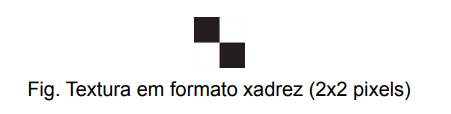
\includegraphics[scale=0.5]{img/xadrez.png}
\end{figure}

\subsection{Aplique uma escala uniforme com fator D (sua variável) no quadrado}

Após a escala uniforme de fator $s = 17$, teremos as coordenadas:

$$[(-17, -17), (17, 17), (-17, 17), (17, -17)]$$

\subsection{Apresente a textura no quadrado (em nova escala) com o parâmetro CLAMP (apenas a ideia via um desenho)}

A ideia da textura com o parâmetro ``clamp'' é de que as "bordas" da textura seja esticada até as bordas da imagem. Como a textura é um xadrez, o quadrado continuaria sendo um xadrez igual ao da figura, com 4 quadrados distintos, porém maior (de tamanho 34x34). Pode ser visto na figura \ref{fig:clamp} - o pontilhado da imagem foi feito apenas para representar as bordas do quadrado, e não existiria no resultado final.


\subsection{Apresente a textura no quadrado (em nova escala) com o parâmetro REPEAT (apenas a ideia via um desenho)}

Com o parâmetro ``repeat'', o xadrez seria replicado várias vezes na imagem. Assim, o padrão se repetiria 17x17 vezes na figura, tendo um total de 34x34 quadrados na imagem, alternando entre preto e branco. Pode ser vista na figura \ref{fig:repeat}. Na figura, está com reticências ($\cdots$) pois a imagem ficaria muito grande.

\begin{figure}[ht!]
	\centering
	\begin{subfigure}{.4\textwidth}
		\centering
		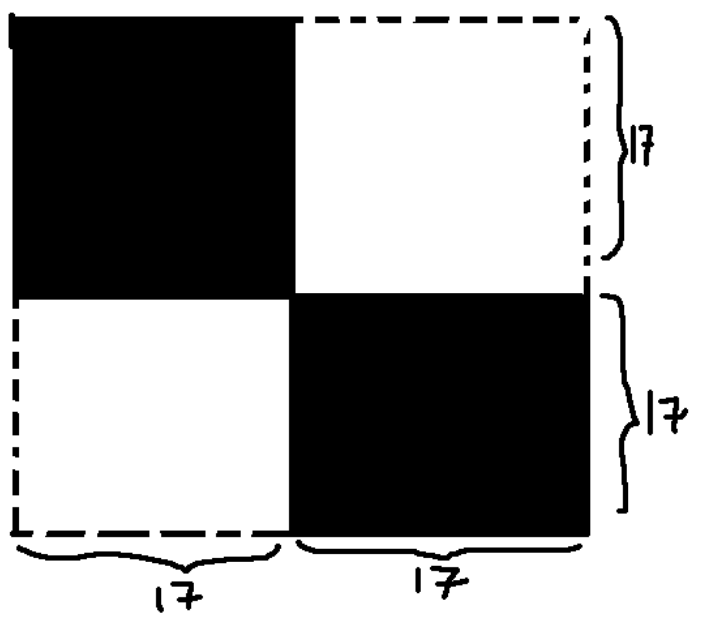
\includegraphics[width=0.8\linewidth]{img/clamp}
		\caption{CLAMP}
		\label{fig:clamp}
	\end{subfigure}
	\begin{subfigure}{.4\textwidth}
		\centering
		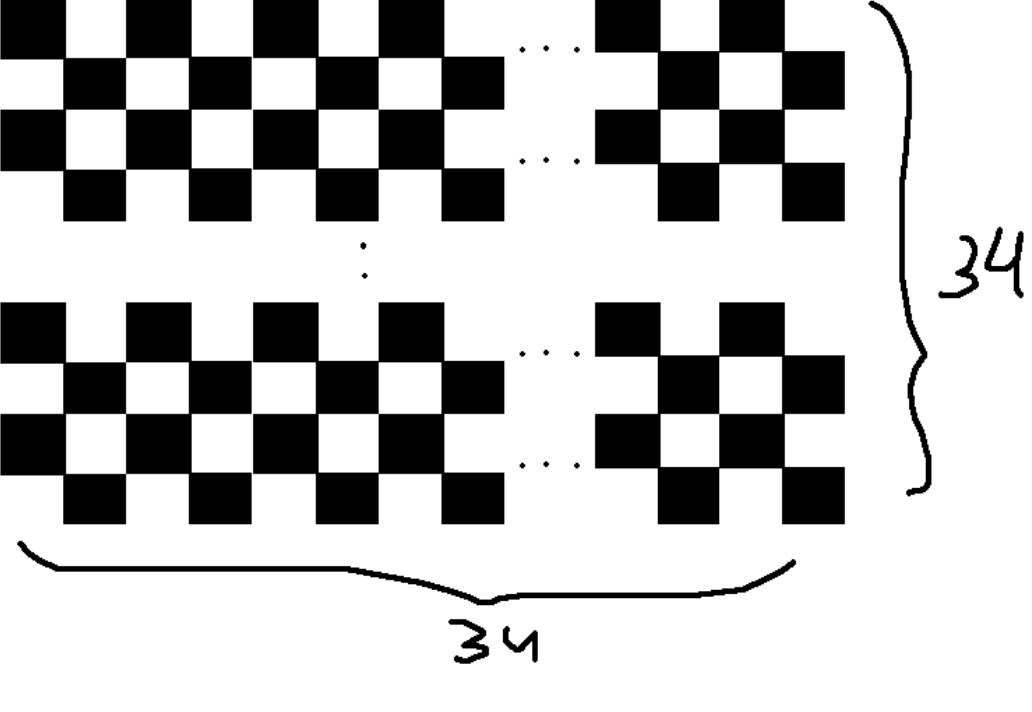
\includegraphics[width=0.9\linewidth]{img/repeat}
		\caption{REPEAT}
		\label{fig:repeat}
	\end{subfigure}
\caption{Textura aplicada no quadrado dado. Fora de escala real.}
\end{figure}

\end{document}